\documentclass{beamer}
\usepackage{graphics}
\usepackage{epsfig}
\usepackage{multicol}
\usepackage{pifont}
\setbeamertemplate{navigation symbols}{}
\newcommand{\RR}{\ensuremath{\mathbb{R}}}
\newcommand{\NN}{\ensuremath{\mathbb{N}}}
\newcommand{\QQ}{\ensuremath{\mathbb{Q}}}
\newcommand{\CC}{\ensuremath{\mathbb{C}}}
\newcommand{\ZZ}{\ensuremath{\mathbb{Z}}}
\newcommand{\TT}{\ensuremath{\mathbb{T}}}
\DeclareMathOperator{\Min}{Min}
\DeclareMathOperator{\Dom}{Dom}
\DeclareMathOperator{\vol}{vol}
\DeclareMathOperator{\Aut}{Aut}
\DeclareMathOperator{\Stab}{Stab}
\DeclareMathOperator{\Sym}{Sym}
\DeclareMathOperator{\Grp}{Grp}
\DeclareMathOperator{\GL}{GL}
\DeclareMathOperator{\Id}{Id}

\begin{document}
\title{Bathymetry smoothing in ROMS: A new approach}
\author{
{\small
\begin{multicols}{2}
\textcolor{red}{\large Mathieu Dutour Sikiri\'c}\\[2mm]
\textcolor{red}{\large Ivica Janekovi\'c}\\[2mm]
\end{multicols}
\begin{center}
\textcolor{red}{\large Milivoj Kuzmi\'c}\\[2mm]
\textcolor{red}{Institute Rudjer Bo\u skovi\'c, Zagreb}
\end{center}
}
}
%\date{\today} 
\date{\empty}

\frame{\titlepage} 

\frame{
  \frametitle{PLAN}

\begin{itemize}
\item[I] Problem set up
\begin{itemize}
\item Sigma coordinates.
\item Slope factors
\item ROMS model and vertical parametrization
\end{itemize}
\item[II] Solution approaches
\begin{itemize}
\item Shapiro, Laplacian filters.
\item Heuristic methods.
\item Linear programming approaches.
\end{itemize}
\item[III] Comparison of selected methods
\begin{itemize}
\item Idealized cases
\item Three grids of the Adriatic
\item Nesting situation.
\end{itemize}
\end{itemize}
}


\frame{
\begin{center}
\begin{tabular*}{7cm}{c}
\\[-0.5cm]
{\Huge
\textcolor{blue}{I. }\textcolor{red}{Problem set up}
}
\end{tabular*}
\end{center}
}


\frame{
  \frametitle{Sigma coordinate systems}

\begin{itemize}
\item One way to deal with varying bathymetry: use $\sigma$-coordinates (\textcolor{blue}{Phillips 1957})
\begin{center}
\begin{minipage}[b]{24mm}
\centering
\resizebox{26mm}{!}{\rotatebox{0}{\includegraphics{OceanPic/SigmaCoordSec.pdf}}}\par
\end{minipage}
\end{center}
\item On every cell $e$ of bathymetry $h(e)$, choose a number $N$ of vertical levels $h(e,k)$ for $1\leq k\leq N$ with $h(e,0)=-h(e)$ and $h(e,N)=0$.
%\item[\textcolor{red}{\ding{224}}] Phillips, N.A., 1957. {\em A coordinate system having some special advantages for numerical forecasting}. Journal of Meteorology 14, 184--185.
\item The differentiation rule of functions in $\sigma$-coordinate is
\begin{equation*}
\left.\displaystyle\frac{\partial f}{\partial x}\right|_z=\left.\displaystyle\frac{\partial f}{\partial x}\right|_{\sigma}+\frac{\partial h}{\partial x} \frac{\partial f}{\partial \sigma}
\end{equation*}
\item This creates a problem for horizontal derivatives, which become a difference of two terms.
The wrong computation of the \textcolor{red}{horizontal pressure gradient} creates artificial currents.
\item \textcolor{blue}{Smagorinsky 1967},
\textcolor{blue}{Janji\'c 1977},
\textcolor{blue}{Mesinger 1982},
\textcolor{blue}{Haney 1991}
\end{itemize}
}


%\frame{
%  \frametitle{Pressure gradient problem}
%
%\begin{itemize}
%\item The differentiation rule of functions in $\sigma$ coordinate is
%\begin{equation*}
%\left.\displaystyle\frac{\partial f}{\partial x}\right|_z=\left.\displaystyle\frac{\partial f}{\partial x}\right|_{\sigma}+\frac{\partial h}{\partial x} \frac{\partial f}{\partial \sigma}
%\end{equation*}
%\item This is creates problem for the computation of the horizontal pressure gradient since the derivative $\frac{\partial p}{\partial x}$ becomes a difference of two terms of same sign.
%\item This is a very old problem (Smagorinsky 1967, Mesinger 1982, Haney 1991).
%\end{itemize}
%}



\frame{
  \frametitle{The slope factors}

\begin{itemize}
\item If $e$ and $e'$ are two adjacent wet cells, then
\begin{equation*}
rx_0(h, e,e')= \frac{|h(e)-h(e')|}{h(e)+h(e')}
\end{equation*}
The maximum over all such pairs is $rx_0(h)$, i.e. the
\textcolor{red}{Beckman \& Haidvogel number}.
\item If the vertical levels of the bathymetries are $h(e,k)$ for $1\leq k\leq N$ then
\begin{equation*}
rx_1(h, e,e',k)=\frac{|h(e,k)-h(e',k)+h(e,k-1)-h(e',k-1)|}{h(e,k)+h(e',k)-h(e,k-1)-h(e',k-1)}.
\end{equation*}
The maximum over $k$ and pairs $e$, $e'$ of adjacent wet cells is $rx_1(h)$.\\
This number is named \textcolor{red}{hydrostatic inconsistency number} or \textcolor{red}{Haney number}.
\end{itemize}
}



\frame{
  \frametitle{Hydrostatic consistency}

\begin{itemize}
\item Denote by $C_k(e)$ the parallelepiped of water between depth $h(e,k-1)$ and depth $h(e,k)$.
\item \textcolor{red}{Hydrostatic consistency} means that if $e$ and $e'$ are any two adjacent cells, then $C_k(e)$ and $C_k(e')$ share a level.
\begin{center}
\begin{minipage}[b]{50mm}
\centering
\resizebox{36mm}{!}{\rotatebox{0}{\includegraphics{OceanPic/HydrostaticInconsistency.pdf}}}\par
\end{minipage}
\end{center}
\item To impose that $C_k(e)$ and $C_k(e')$ share a level is equivalent to $rx_1(h, e, e', k)\leq 1$ (\textcolor{blue}{Rousseau and Pham 1971}, \textcolor{blue}{Mesinger 1982}, \textcolor{blue}{Haney 1991}).
\item This requirement is very strong and almost impossible to fulfill.
\end{itemize}
}





\frame{
  \frametitle{What are the right values of $rx_1$, $rx_0$}

There is no general agreement on this question
\begin{itemize}
\item The factor which matters for the horizontal pressure gradient is the Haney number $rx_1(h)$.
\item It is extremely difficult to achieve $rx_1(h)\leq 1$.
\item In \textcolor{blue}{Mellor-Ezer-Oey, 1994} it is argued that the HPG error is not very important and disappears after running the model for some time.
\item \textcolor{blue}{Kliem-Pietrzak, 1999} contests this for the Skagerrak region.
\item \textcolor{blue}{Sasha Shchepetkin, 2008} says that $rx_1(h)\leq 3$ is ``safe'', $rx_1(h)\simeq 5$ is ``common'' and $rx_1(h)\geq 8$ is ``insane''.
\item \textcolor{blue}{Kate Hedstr\"om, 2008} reported no problem with $rx_1(h)\simeq 16$.
%\item There are contrary argument about the importance of pressure gradient error by \textcolor{blue}{Mellor-Ezer-Oey 1994} and \textcolor{blue}{Kliem-Pietrzak, 1999}.
\item We experienced blow ups with grids with $rx_1(h)\geq 9$.
\item We call a grid \textcolor{red}{numerically stable} if $rx_1(h) \leq 6$.
\end{itemize}
}


\frame{
  \frametitle{The ROMS model}

\begin{itemize}
\item ROMS is an hydrostatic regional $\sigma$-coordinate ocean model with several advection scheme.
\item There are three versions of ROMS
\begin{itemize}
\item ROMS AGRIF maintained by \textcolor{blue}{Debreu} (public).
\item ROMS UCLA maintained by \textcolor{blue}{Shchepetkin} (non public).
\item ROMS Rutgers maintained by \textcolor{blue}{Arango} (public, main version).
\end{itemize}
\item ROMS Rutgers has possibility of coupling with the SWAN model, adjoint and tangent linear functionalities for strong 4dvar, weak 4dvar.
\item ROMS AGRIF and ROMS UCLA have built in nesting capabilities. ROMS UCLA has the highest speed and there exists a non hydrostatic version of ROMS UCLA.
\end{itemize}
}

\frame{
  \frametitle{Vertical parametrization in ROMS}
\begin{itemize}
\item The ROMS vertical parametrization depends on three parameters $hc$, $\theta_s$, $\theta_b$
\begin{equation*}
h(e,k)=s_w(k) hc + (h(e) - hc) c_w(k).
\end{equation*}
$hc$ is the thermocline parameter and it is lower than the minimal
depth of the model.
\item The vertical parametrization function depends on $\theta_s$ and $\theta_b$ and is $s_w(k)=-\frac{k}{N}$.
\begin{equation*}
c_w(k)=(1-\theta_b)\frac{\sinh \theta_s s_w(k)}{\sinh \theta_s}
+\theta_b \left\{\frac{\tanh \theta_s(s_w(k) + \frac{1}{2})}{2 \tanh \frac{\theta_s}{2}}-\frac{1}{2}   \right\}
\end{equation*}
This formula is relatively arbitrary (\textcolor{blue}{Song, 1994}) and another one may work just as well.
\item If $hc=0$ then we have $h(e,k)=h(e)c_w(k)$ and we get
\begin{equation*}
rx_1(h)=\max_{1\leq k\leq N} \frac{c_w(k) + c_w(k-1)}{c_w(k) - c_w(k-1)} rx_0(h)
\end{equation*}
%\item[\textcolor{red}{\ding{224}}]
%Song, Y., Haidvogel, D.B., 1994.
%{\em A semi-implicit ocean circulation model using a generalized topography-following coordinate system}.
%Journal of Computational Physics 115, 228--244.
\end{itemize}
}



\frame{
  \frametitle{Choice of vertical stratification}

\begin{itemize}
\item If one wants only to minimize $rx_1$, then the choice is $\theta_b=0$ and $\theta_s$ high, i.e. concentrate the vertical levels on the surface.\\
But we cannot concentrate the levels too much on the surface so it is recommended to have $\theta_s$ at most $7$.
\item If the bottom boundary layers is a zone of interest, then a nonzero value of $\theta_b$ has to be chosen.
\item The number of vertical levels is the main constraints. It limits the computational possibilities and the error pressure gradient.
\end{itemize}
\begin{center}
\begin{minipage}[b]{1.7cm}
\centering
\epsfig{width=16mm, file=OceanPic/FileN20_thetaS3_thetaB0_35-crop.pdf}
\end{minipage}
\begin{minipage}[b]{1.7cm}
\centering
\epsfig{width=16mm, file=OceanPic/FileN20_thetaS3_thetaB0_8-crop.pdf}
\end{minipage}
\begin{minipage}[b]{1.7cm}
\centering
\epsfig{width=16mm, file=OceanPic/FileN20_thetaS3_thetaB0-crop.pdf}
\end{minipage}
\begin{minipage}[b]{1.7cm}
\centering
\epsfig{width=16mm, file=OceanPic/FileN50_thetaS7_thetaB0-crop.pdf}
\end{minipage}
\end{center}

}



\frame{
  \frametitle{Possible ways to deal with the problem}

If the bathymetry is too steep then this causes instabilities and inaccuracies.
Some possible ways to deal with it:
\begin{itemize}
\item Use a high order pressure gradient scheme (\textcolor{blue}{Chu \& Fan, 1997, 1998, 2003})
(\textcolor{red}{computational price})
\item Adjust the vertical stratification, i.e. $s_w$, $c_w$ and in case of ROMS $\theta_s$, $\theta_b$ (\textcolor{red}{modelling choices}).
\item Decrease the number $N$ of vertical levels (\textcolor{red}{less realistic})
\item Make the horizontal grid finer (\textcolor{red}{computational price}).
\item Smooth the bathymetry (\textcolor{red}{less realistic}).
\item Use a $z$- or generalized coordinate system (\textcolor{red}{change of model}).
\end{itemize}
We consider the smoothing methods to reduce the magnitude of the problem.
}




\frame{
\begin{center}
\begin{tabular*}{7cm}{c}
\\[-0.5cm]
{\Huge
\textcolor{blue}{II. }\textcolor{red}{Solution approaches}
}
\end{tabular*}
\end{center}
}


\frame{
  \frametitle{The goal}

\begin{itemize}
\item The grid is build in the following way:
\begin{itemize}
\item Build an initial grid using coastline informations.
\item Choose the parameters $N$, $\theta_s$, $\theta_b$ and $hc$.
\item Find the initial bathymetry $h^{obs}$ from existing data set (NOAA, Gshhs, Gebco, etc.)
\item Determine the smoothed bathymetry $h$.
\end{itemize}
\item Requirements:
\begin{itemize}
\item $rx_0(h)$ and $rx_1(h)$ low.
\item The ``distance'' between $h$ and $h^{obs}$ small.
\item $h$ should have the same physical characteristics as $h^{obs}$.
\end{itemize}
\item For a given $r$ and $h^{obs}$, we will present methods to get $h$
with $rx_0(h) \leq r$.
\item The analysis for $rx_1$ works similarly.
\end{itemize}
}


\frame{
  \frametitle{Why optimize with $rx_0$?}

\begin{itemize}
\item It is less expensive computationally than optimizing with $rx_1$.
\item If the depth is sufficiently large then the relation
\begin{equation*}
rx_1(h)=\max_{1\leq k\leq N} \frac{c_w(k) + c_w(k-1)}{c_w(k) - c_w(k-1)} rx_0(h)
\end{equation*}
is almost exact.
\item For the interesting domain $rx_1\leq 6$, the result of optimization with $rx_1$ is at most $5\%$ different from optimizing with respect to $rx_0$.
\item The error pressure gradient is more important in region of high density differences. Those are typically regions of moderate to high depth.
\end{itemize}
}


\frame{
  \frametitle{The grid problem}
\begin{itemize}
\item The observed bathymetry is available on a grid different from the one of the model.
\item We have two possible situations:
\begin{itemize}
\item The observations are sparser than the model bathymetry.
\item The resolution of the observations is better than the resolution of the model.
\end{itemize}
\item In the first situation, the solution is necessarily to interpolate
the bathymetry from the available observations to the model grid. If the 
observations have no regular structure (ship, ...) then the best is to
use natural neighbor interpolation (\textcolor{blue}{Sibson 1981}) with the
program \textcolor{red}{{\tt nnbathy}} by \textcolor{blue}{Pavel Sakov, 2006}.
\item In the Adriatic, actually we have high resolution bathymetry and we
are in the latter situation.
\end{itemize}
}

\frame{
  \frametitle{The averaging procedure}

\begin{itemize}
\item When we have more bathymetry observations than necessary for the model, then we take the average over wet cells of the observations that belong to them.
\item Another strategy is to use the Shapiro filter several times and then to interpolate to the grid of the model.
\item The problem is that by doing this we smooth the bathymetry and reduce the slope factor even when this is not needed.
\item The HPG problem is a model problem and so it should be treated at level of grid of the model.
\item The right method is thus:
  \begin{itemize}
  \item First compute of the model at the grid level.
  \item Then smooth it, to reduce the HPG error.
  \end{itemize}

\end{itemize}
}



\frame{
  \frametitle{The Shapiro filter}

\begin{itemize}
\item It is a filter designed to smooth out fast waves in finite
difference models (\textcolor{blue}{Shapiro 1975}).
\item It was not designed for smoothing out the bathymetry but it is
still frequently used to smooth out bathymetry variations.
\item Every ROMS version has its own version of the filter.
\begin{itemize}
\item ROMS AGRIF has a Shapiro filter applied to the logarithm of the bathymetry first in $x$-direction and then in $y$-directions.
\item ROMS UCLA has a Shapiro filter applied to the logarithm of the bathymetry with a more complex stencil.
\item ROMS Rutgers has a Shapiro filter applied in $x$- and $y$-directions only to the points where the slope factor is not correct.
\end{itemize}
\item The POM model has its own filter named ``Gaussian filter''.
\end{itemize}
}

\frame{
  \frametitle{The Shapiro filter of ROMS Rutgers}

\begin{itemize}
\item It is applied to the bathymetry in the following way:
\begin{flushleft}
$h \textcolor{red}{\leftarrow} h^{obs}$\\
\textbf{while} $rx_0(h) > r$ \textbf{do}\\
\hspace{2ex} $h' \textcolor{red}{\leftarrow}$ Shapiro filtering of $h$ on $x$ direction.\\
\hspace{2ex} \textbf{for} $e$ in wet cells \textbf{do}\\
\hspace{2ex} \hspace{2ex} \textbf{if } $rx_o(h, e)>r$ \textbf{then}\\
\hspace{2ex} \hspace{2ex} \hspace{2ex} $h(e) \textcolor{red}{\leftarrow} h'(e)$\\
\hspace{2ex} \hspace{2ex} \textbf{end if}\\
\hspace{2ex} \textbf{end for}\\
\hspace{2ex} Do the same in $y$ direction\\
\textbf{end do}
\end{flushleft}
\item For some bathymetries the Shapiro filter converges to $h$ with $rx_0(h) > r$ and thus the program never ends.
\item The best Shapiro filter of all $3$ is the one of ROMS UCLA.
\end{itemize}
}






\frame{
  \frametitle{Laplacian filter}

\begin{itemize}
\item It works in the following way:
\begin{itemize}
\item start with $h=h^{obs}$.
\item If $rx_0(h, e) > r$ we do:
\begin{equation*}
h(e)\textcolor{red}{\leftarrow} h(e)+\frac{1}{2N(e)} \sum_{e'\in N(e)} \{ h(e')-h(e)\}
\end{equation*}
with $N(e)$ the set of wet cells adjacent to the wet cell $e$.
\item Iterate until $rx_0(h)\leq r$.
\end{itemize}
\item This filter is more stable than Shapiro filter, but there is a still a problem of having the program end.
\item Shapiro filter and Laplacian filter are very frequently used but they are not very good methods.
\end{itemize}
}





\frame{
  \frametitle{The Martinho \& Batteen (MB) scheme}

\begin{itemize}
\item Whenever the slope is not correct the chosen solution
(\textcolor{blue}{Martinho \& Batteen 2006}) is to
increase the bathymetry.
\begin{itemize}
\item Start with $h=h^{obs}$
\item If
\begin{equation*}
\frac{h(e) - h(e')}{h(e) + h(e')} > r\quad{\rm then} \quad h(e')\textcolor{red}{\leftarrow} \frac{1-r}{1+r}h(e)
\end{equation*}
\item All pairs $(e, e')$ are considered iteratively until the slope factor is correct. The result is independent of the order of operations.
\end{itemize}
%\item[\textcolor{red}{\ding{224}}] Martinho, A.S., Batteen, M.L., 2006. {\em On reducing the slope parameter in terrain following numerical ocean models}. Ocean Modelling 13, 166--175.
\item They also proposed to preserve the volume by replacing the bathymetry $h$ obtained by their method by 
\begin{equation*}
h\textcolor{red}{\leftarrow} h \frac{\vol h^{obs}}{\vol h}.
\end{equation*}
This method works because $rx_0(\alpha h)=rx_0(h)$.
%\item \textcolor{red}{Note}: the strategy of reducing the bathymetry does not work efficiently.
\end{itemize}
}

\frame{
  \frametitle{The bathymetry decreasing scheme}
\begin{itemize}
\item Whenever the slope is not correct the chosen solution
is to decrease the bathymetry.
\begin{itemize}
\item Start with $h=h^{obs}$
\item If
\begin{equation*}
\frac{h(e) - h(e')}{h(e) + h(e')} > r\quad{\rm then} \quad h(e)\textcolor{red}{\leftarrow} \frac{1+r}{1-r}h(e')
\end{equation*}
\item All pairs $(e, e')$ are considered iteratively until the slope factor is correct. The result is independent of the order of operations.
\end{itemize}
\item This filter can help for initialization problems when the initial state
has to be taken from measured or initial values and not from extrapolated
values from a nearest point.

\end{itemize}
}

\frame{
  \frametitle{The Mellor-Ezer-Oey (MEO) scheme}

\begin{itemize}
\item (\textcolor{blue}{Mellor 1994}) If we want to preserve volume, then another scheme is possible.
\begin{itemize}
\item If we have 
\begin{equation*}
\frac{h(e) - h(e')}{h(e) + h(e')} > r
\end{equation*}
then we write
\begin{equation*}
h(e)\textcolor{red}{\leftarrow} h(e)-\frac{V(e,e')}{A(e)}\quad {\rm and}\quad h(e')\textcolor{red}{\leftarrow} h(e')+\frac{V(e,e')}{A(e')}
\end{equation*}
with $V(e,e')$ adjusted so that  $\frac{h(e) - h(e')}{h(e) + h(e')}=r$ and $A(e)$, $A(e')$ the area of wet cell $e$, $e'$.
\item All pairs $(e,e')$ of adjacent wet cells are considered iteratively until the bathymetry is correct.
\end{itemize}
\item A priori, the final bathymetry depends from the order of the operations.
%\item[\textcolor{red}{\ding{224}}] Mellor, G.L., Ezer, T., Oey, L.-Y., 1994. {\em The pressure gradient conundrum of Sigma coordinate Ocean models}. Journal of Atmospheric and Oceanic Technology 11, 1126--1134.
\end{itemize}
}




\frame{
  \frametitle{Definition of linear programs}

\begin{itemize}
\item A \textcolor{red}{linear program} is the problem of maximizing a linear function $f(x)$ over a set ${\mathcal P}$ defined by linear inequalities.
\begin{equation*}
{\mathcal P}=\{ x\in \RR^d \quad{\rm such~that} \quad f_i(x) \geq b_i\}
\end{equation*}
with $f_i$ linear and $b_i\in \RR$.
%\item The sets ${\mathcal P}$ are called \textcolor{red}{polyhedral}.
\item The solution of linear programs is attained at vertices of ${\mathcal P}$.
\item There are two classes of solution methods:
\begin{center}
\begin{minipage}[b]{38mm}
\centering
\resizebox{30mm}{!}{\rotatebox{0}{\includegraphics{OceanPic/SimplexMethod.pdf}}}\par
Simplex method
\end{minipage}
\begin{minipage}[b]{38mm}
\centering
\resizebox{30mm}{!}{\rotatebox{0}{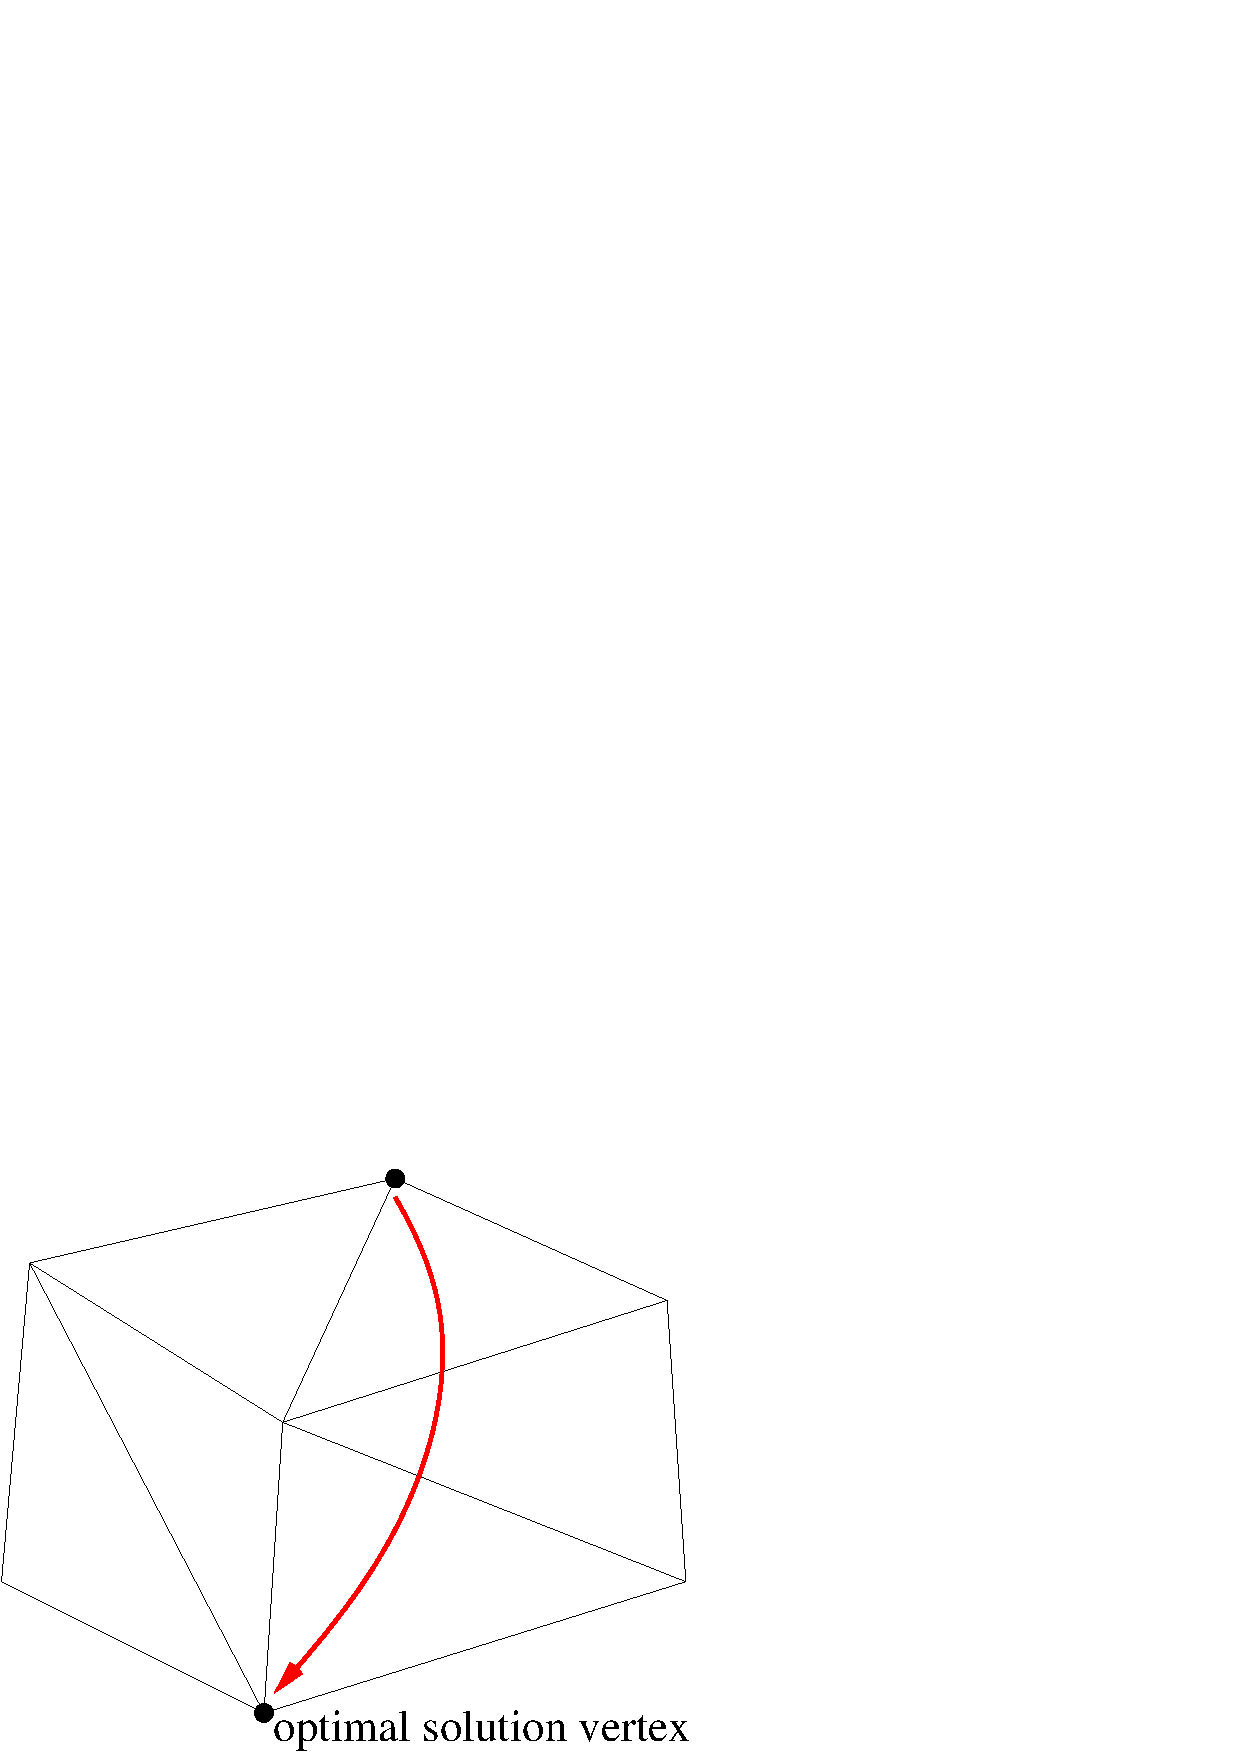
\includegraphics{OceanPic/InteriorPM.pdf}}}\par
Interior point method
\end{minipage}
\end{center}


\end{itemize}
}




\frame{
  \frametitle{Linear programming methods}

\begin{itemize}
\item The inequality $rx_0(h, e, e')\leq r$ corresponds to:
\begin{equation*}
-r (h(e) + h(e'))\leq h(e)-h(e') \leq r (h(e) + h(e'))
\end{equation*}
\item We introduce some auxiliary variable $\delta(e)$ with 
\begin{equation*}
|h(e)-h^{obs}(e)| \leq \delta(e) \quad {\rm i.e.}\quad \pm(h(e)-h^{obs}(e))\leq \delta(e)
\end{equation*}
\item And we minimize
\begin{equation*}
\sum_{e} \delta(e) \quad{\rm that~is} \quad \sum_e |h(e)-h^{obs}(e)|.
\end{equation*}
\item There are many possible variants, which are still in the linear programming paradigm:
\begin{itemize}
\item Preserve the total volume of the basin.
\item Have a different objective function.
\item Impose only positive/negative corrections at some points.
\item Impose maximum amplitude condition.
\item Fix some points (nested applications)
\end{itemize}
\end{itemize}
}

\frame{
  \frametitle{Linearized Mellor-Ezer-Oey (LMEO) scheme}

\begin{itemize}
\item For all pair $(e,e')$ of adjacent wet cells $e$, $e'$ consider the operations.
\begin{equation*}
h(e)\textcolor{red}{\leftarrow} h(e)-\frac{V(e,e')}{A(e)}\quad {\rm and}\quad h(e')\textcolor{red}{\leftarrow} h(e')+\frac{V(e,e')}{A(e')}
\end{equation*}
\item For a set of volumes $V(e,e')$, consider the resulting bathymetry $h$ obtained from $h^{ave}$.
\item The objective function is 
\begin{equation*}
\sum_{(e,e')} |V(e,e')|
\end{equation*}
\item This method is supposed to be a reformulation of Mellor-Ezer-Oey where we minimize the volumes $V(e,e')$ involved.

\end{itemize}
}



%\frame{
%  \frametitle{Solution methods}
%
%\begin{itemize}
%\item There are two classes of solution method for solving linear programs:
%\item Simplex method (take one vertex and optimize step by step).
%\item Interior Point methods (take an interior point and make it nearer to the optimal solution)
%\end{itemize}
%}







\frame{
\begin{center}
\begin{tabular*}{7cm}{c}
\\[-0.5cm]
{\Huge \textcolor{blue}{III. }\textcolor{red}{Comparison}}\\
{\Huge \textcolor{red}{of selected methods}}
\end{tabular*}
\end{center}
}

\frame{
  \frametitle{Idealized cases: Sill}
\begin{center}
\begin{minipage}[b]{5.3cm}
\centering
\epsfig{width=50mm, file=OceanPic/1dimSill_lsmo_nega_lapl0_20-crop.pdf}\par
\end{minipage}
\begin{minipage}[b]{5.3cm}
\centering
\epsfig{width=50mm, file=OceanPic/1dimSill_MB_LinProg0_20-crop.pdf}\par
\end{minipage}
\end{center}
\begin{itemize}
\item We should avoid the bathymetry decreasing method.
\end{itemize}
}




\frame{
  \frametitle{Idealized cases: Pit}

\begin{center}
\begin{minipage}[b]{5.3cm}
\centering
\epsfig{width=50mm, file=OceanPic/1dimPit_lsmo_nega_lapl0_20-crop.pdf}\par
\end{minipage}
\begin{minipage}[b]{5.3cm}
\centering
\epsfig{width=50mm, file=OceanPic/1dimPit_MB_LinProg0_20-crop.pdf}\par
\end{minipage}
\end{center}
\begin{itemize}
\item The Martinho \& Batteen method is good for preserving the depth of the pits.
\end{itemize}
}


\frame{
  \frametitle{Idealized cases: Shelf break}

\begin{center}
\begin{minipage}[b]{5.3cm}
\centering
\epsfig{width=50mm, file=OceanPic/1dimShelf_lsmo_nega_lapl0_20-crop.pdf}\par
\end{minipage}
\begin{minipage}[b]{5.3cm}
\centering
\epsfig{width=50mm, file=OceanPic/1dimShelf_MB_LinProg0_20-crop.pdf}\par
\end{minipage}
\end{center}
\begin{itemize}
\item LP does a better job of preserving the shelf break.
\end{itemize}
}



\frame{
  \frametitle{Idealized cases (volume preserving): Sill}

\begin{center}
\begin{minipage}[b]{5.3cm}
\centering
\epsfig{width=50mm, file=OceanPic/1dimSill_posVol_LinVol0_20-crop.pdf}\par
\end{minipage}
\begin{minipage}[b]{5.3cm}
\centering
\epsfig{width=50mm, file=OceanPic/1dimSill_secsch_mellor0_20-crop.pdf}\par
\end{minipage}
\end{center}
\begin{itemize}
\item MEO (Mellor-Ezer-Oey) gives the same result as LMEO (Linearized Mellor-Ezer-Oey).
\item MB method spread the perturbation globally.
\end{itemize}

}



\frame{
  \frametitle{Idealized cases (volume preserving): Pit}

\begin{center}
\begin{minipage}[b]{5.3cm}
\centering
\epsfig{width=50mm, file=OceanPic/1dimPit_posVol_LinVol0_20-crop.pdf}\par
\end{minipage}
\begin{minipage}[b]{5.3cm}
\centering
\epsfig{width=50mm, file=OceanPic/1dimPit_secsch_mellor0_20-crop.pdf}\par
\end{minipage}
\end{center}
\begin{itemize}
\item The MB method is again better for the pits but the perturbation is global to the basin.
\end{itemize}
}


\frame{
  \frametitle{Idealized cases (volume preserving): Shelf break}

\begin{center}
\begin{minipage}[b]{5.3cm}
\centering
\epsfig{width=50mm, file=OceanPic/1dimShelf_posVol_LinVol0_20-crop.pdf}\par
\end{minipage}
\begin{minipage}[b]{5.3cm}
\centering
\epsfig{width=50mm, file=OceanPic/1dimShelf_secsch_mellor0_20-crop.pdf}\par
\end{minipage}
\end{center}
\begin{itemize}
\item The Linearized Mellor-Ezer-Oey method gives a worse result than the MEO method. We should avoid LMEO.
\item LP is very near to the MEO method.
\end{itemize}

}








\frame{
  \frametitle{The Adriatic Sea}
\begin{center}
\begin{minipage}{60mm}
\centering
\epsfig{height=60mm, file=OceanPic/RawBathyContourRect_V2_norect-crop.pdf}\par
%RawBathyContourRect.pdf
\end{minipage}
\end{center}
\hspace{-2.7mm}\begin{itemize}
\item The bathymetry is highly varying and the coastline is diverse.
\item We chose three grids $160\times 60$, $127\times 368$, $271\times 751$
\end{itemize}
}



\frame{
  \frametitle{Hydrostatic consistency \& numerical stability}

\begin{center}
\hspace{-1.1cm}\begin{minipage}[b]{3.8cm}
\centering
%\hspace{-1cm}
\epsfig{height=40mm, file=OceanPic/ADRIA02_Hydrostatic-crop.pdf}\par
$60\times 160$
\end{minipage}
\hspace{0.2cm}
\begin{minipage}[b]{3.7cm}
\centering
%\hspace{-0.5cm}
\epsfig{height=40mm, file=OceanPic/NCOM2_Hydrostatic-crop.pdf}\par
$127\times 368$
\end{minipage}
\hspace{0.1cm}
\begin{minipage}[b]{3.5cm}
\centering
\epsfig{height=40mm, file=OceanPic/NCOM1_Hydrostatic-crop.pdf}\par
$271\times 751$
\end{minipage}
\end{center}
The regions of hydrostatic consistency \& numerical stability ($rx_1(h, e)\leq 1$ in light blue), hydrostatic inconsistency \& numerical stability ($1\leq rx_1(h, e)\leq 5$ in dark blue) and hydrostatic inconsistency \& numerical instability ($rx_1(h, e)\geq 5$ in red)
}



\frame{
  \frametitle{Average amplitude of bathymetry modification}

\begin{center}
\begin{minipage}[b]{5.3cm}
\centering
\epsfig{height=49mm, file=OceanPic/TOP7samp_ADRIA02_Various-crop.pdf}\par
$60\times 160$
\end{minipage}
\begin{minipage}[b]{5.3cm}
\centering
\epsfig{height=49mm, file=OceanPic/TOP7samp_NCOM2_Various-crop.pdf}\par
$127\times 368$
\end{minipage}
\end{center}
The average amplitude of bathymetry modification (m) in terms for bathymetry smoothing methods
}


\frame{
  \frametitle{Average variation of bathymetry}


\begin{center}
\begin{minipage}[b]{5.3cm}
\centering
\epsfig{height=52mm, file=OceanPic/TOP7samp_ADRIA02_Gradient-crop.pdf}\par
$60\times 160$
\end{minipage}
\begin{minipage}[b]{5.3cm}
\centering
\epsfig{height=52mm, file=OceanPic/TOP7samp_NCOM2_Gradient-crop.pdf}\par
$127\times 368$
\end{minipage}
\end{center}
The average variation of the bathymetry (m) from wet cell
to wet cell for bathymetry smoothing methods in terms of $rx_0(h)$
}



\frame{
  \frametitle{Average amplitude of bathymetry modification}

\begin{center}
\begin{minipage}[b]{5.3cm}
\centering
\epsfig{height=52mm, file=OceanPic/TOP7samp_ADRIA02_VolVarious-crop.pdf}\par
$60\times 160$
\end{minipage}
\begin{minipage}[b]{5.3cm}
\centering
\epsfig{height=52mm, file=OceanPic/TOP7samp_NCOM2_VolVarious-crop.pdf}\par
$127\times 368$
\end{minipage}
\end{center}
The average amplitude of bathymetry modification (m) in term of $rx_0$ for volume preserving smoothing methods
}

\frame{
  \frametitle{Average variation of the bathymetry}

\begin{center}
\begin{minipage}[b]{5.3cm}
\centering
\epsfig{height=50mm, file=OceanPic/TOP7samp_ADRIA02_VolGradient-crop.pdf}\par
$60\times 160$
\end{minipage}
\begin{minipage}[b]{5.3cm}
\centering
\epsfig{height=50mm, file=OceanPic/TOP7samp_NCOM2_VolGradient-crop.pdf}\par
$127\times 368$
\end{minipage}
\end{center}
The average variation of the bathymetry (m) from wet cell
to wet cell for bathymetry smoothing methods preserving volume
in terms of $rx_0$
}


\frame{
  \frametitle{Effect of smoothing}

\begin{itemize}
\item The need for smoothing decrease when the horizontal grid is finer:
\begin{center}
\begin{tabular}{|c|c|}
\hline
grid             & volume perturbed\\\hline
$60\times 160$   & $322$km${}^3$\\\hline
$127\times 368$  & $20$km${}^3$\\\hline
$271\times 751$  & $7.2$km${}^3$\\\hline
\end{tabular}
\end{center}
\item Time runs:
\begin{itemize}
\item Heuristic methods take at most $20$ seconds for smoothing.
\item Shapiro and Laplacian do not take more than a few minutes in general.
\item Linear programming takes more time $5$ min for $60\times 160$, $1$ hour for $127\times 368$ and $1$ day for $271\times 751$.
\end{itemize}
\item Having the right bathymetry in the model can be the key to correct modelization:
\begin{itemize}
\item[\textcolor{red}{\ding{224}}] Batteen et al., 2007. {\em A process oriented modelling study of the coastal Canary and Iberian Current system}. Ocean modelling 18, 1--36.
\end{itemize}

\end{itemize}
}



\frame{
  \frametitle{Stability of solutions}

What happens if one perturb by an infinitesimal quantity the observed bathymetry and/or the slope factor?
\begin{itemize}
\item Heuristic methods (MEO, MB) are continuous.
\item Shapiro filter and Laplacian filter methods are not continuous.
\item Linear programming methods are not continuous since there are possible hoppings from one vertex to an adjacent one.
\end{itemize}
In practice during $0.01$ increments to $rx_0$ for the $127\times 368$ grid,
\begin{center}
\begin{tabular}{c|c|c|}
method      & average change & maximal change\\\hline
MB          & $5.4$cm & $7.8$m\\
LP          & $5.2$cm & $13.8$m\\
Laplacian   & $6.4$cm & $23$m\\
Shapiro     & $40cm$  & $28$m\\
\end{tabular}
\end{center}
}


\frame{
  \frametitle{Nested grid situations}

\begin{itemize}
\item Suppose we have a grid of say $2km$ of resolution, another grid of $700m$ around Rovinj region is embedded in it in a $1$-way coupling situation.
We want the bathymetry of the embedded grid to coincide with the bathymetry of the embedded grid on the boundaries.
\item The method is the following.
\begin{enumerate}
\item Compute the raw bathymetry $h^{raw}$ of the embedded grid using averaging operations.
\item Interpolate the bathymetry of the $2km$ grid to the $700m$ grid.
\item Fix the boundary values of the bathymetry of the $700m$ grid to be interpolated values.
\item Smooth $h^{raw}$ by specifying no change of boundary values.
\end{enumerate}


\end{itemize}
}







\frame{
  \frametitle{Conclusions}

\begin{itemize}
\item Shapiro and Laplacian filter should be avoided since they create large perturbation of the bathymetry.
\item Heuristic methods like Martinho-Batteen, Mellor-Ezer-Oey work relatively well.
\item If $rx_0(h)\leq 0.2$ is needed, then linear programming might be what you need.
%\item There are many possible variants one can build on this to optimize the bathymetry.
\item All programs (in matlab) for optimizing over $rx_0$ or $rx_1$ are available from
\begin{center}
{\small \url{http://drobilica.irb.hr/~mathieu/Bathymetry/index.html}}
\end{center}

\end{itemize}
}





%\frame{
%\vspace{1.5cm}
%\begin{center}
%{\Huge \textcolor{red}{T}\textcolor{blue}{H}\textcolor{green}{A}\textcolor{blue}{N}\textcolor{red}{K}}\\[1cm]
%{\Huge \textcolor{red}{Y}\textcolor{blue}{O}\textcolor{red}{U}}
%\epsfig{file=plit-gal10.eps, height=5.5cm}
%\end{center}
%}






\end{document}
